\documentclass[a4paper, twocolumn, twoside, 12pt]{article}
\usepackage[utf8]{inputenc}
\usepackage[english]{babel}
\usepackage{graphicx}
\usepackage{color}
\usepackage{setspace}
\usepackage{hyperref}
\usepackage{url}
\usepackage[left=1cm, right=1cm, top=1cm, bottom=2cm]{geometry}

\setstretch{0.8}
\setlength{\parindent}{2em}
%\setlength{\parskip}{0em}
%\vspace{1ex}

\begin{document}

\title{\textbf{Simulation and Analysis of Propagation Models  \\Using NS3}\vspace{-0.6em}}

\author{Samuel Anamah
\\ samuel\_segun.anamah@smail.th-koeln.de
\\ MaCSN TH Koeln\vspace{-1em}}
\date{}
\maketitle

\textbf{\textit{Abstract---}This paper analysis the simulation of wireless Adhoc 802.11n point to point network and considered how different propagation models are implemented in ns-3 with respect to how these models influence or affects the outcome of a WiFi simulation. Also, this paper tests how varying distance impacts ns-3 WiFi simulation. Although, there are several propagation models, we will only consider five propagation models in this paper.}

\maketitle
\section{Introduction \vspace{-0.2em}}
A wireless ad hoc network (WANET) is a type of local area network (LAN) that is built spontaneously to enable two or more wireless devices to be connected to each other without requiring typical network infrastructure equipment, such as a wireless router or access point. When Wi-Fi networks are in ad hoc mode, each device in the network forwards data that is not intended for itself to the other devices [1]. Throughput, signal strength and distance are some majors consign when it comes to WANET.

For this study, Network Simulator 3 (ns3.30 and ns3.32) was used. This tool will be used to simulate five different propagation loss models.  Namely, Friis Propagation Loss Model, Fixed Rss Loss Model, Three Log Distance Propagation Loss Model, Two Ray Ground Propagation Loss Model and Nakagami Propagation Loss Model. The propagation loss model is used to determine the wireless signal strength at the receivers for any packet being transmitted by a single transmitter[2].

\section{Methodology \vspace{-0.2em}}
NS3 was used to simulate two WiFi nodes using the IEEE802.11n standard operating in the Unlicensed National Information Infrastructure (U-NII) 5 GHz Band. Both WiFi nodes were configured to use the simple Adhoc WiFi MAC. The distance between the nodes was varied.  The output power of the WiFi cards was fixed to 10 dBm and an omnidirectional antenna with 1 dBi was used on both nodes. IP and UDP was used at the upper layers to generate artificial UDP traffic with an application layer packet size of 1450 Bytes, a data-rate of 75 Mbps and a channel width of 160 MHz.

In order to achieve the set objectives, the necessary modules for the program were imported into the source code in order for the associated commands to work. The program provides the possibility for users to input some command line arguments like simulation time, preferred propagation model, distance between the WiFi nodes and verbose.

Firstly, a container was created to host the two nodes that will be created using \textit{NodeContainer}. Next, the \textit{WiFiHelper} was called to set the wifi standard to “WIFI\_STANDARD\_80211n\_5GHZ” or “WIFI\_PHY\_STANDARD\_80211n\_5GHZ” and to set the remote station manager to “MinstrelHtWifiManager”. \textit{YansWifiPhyHelper} named wifiPhy class was used to build the physical layer. The transmission power start and end (TxPowerStart and TxPowerEnd), transmission gain (TxGain), reception gain (RxGain), channel width (ChannelWidth), frequency (Frequency) and transmission power level (TxPowerLevels) were set as stated above. \textit{YansWifiChannelHelper} named wifiChannel was used to create a loop to specify the preferred propagation loss model \textbf{(FriisPropagationLossModel,  FixedRssLossModel, ThreeLogDistancePropagationLossModel, TwoRayGroundPropagationLossModel or Nakagami)} as provided by the user in the command line argument. \textit{WifiMacHelper} named wifiMac was used to set the Adhoc type to "AdhocWifiMac". \textit{NetDeviceContainer} named apDevices was used to install "wifiPhy" and "wifiMac" on the nodes. Also, the nodes were positioned using \textit{MobilityHelper} object. The mobility model used is the Constant Position Mobility Model.

Next, the internet stack was created using \textit{InternetStackhelper} and was installed on the nodes to provide layer 3 connectivity. The nodes were assigned network address 192.168.170.64/29 and was stored in apNodeInterface. The layer4 UDP flow was created using \textit{UdpServerHelper} which was used to create the server application and also to install it on the first node with a specified start and stop time.  The client application was created and installed using \textit{OnOffHelper} on the second node.

Flow monitor was implemented using \textit{FlowMoniorHelper} to show and monitor how packets flow from the client to the server and to measure the performance of network protocols [3].

Finally, the simulation is set to stop at the specified time and the output is printed afterwards, by displaying the flow(s), propagation model, transmission packets, transmission bytes, transmission offered (throughput at transmission), reception packets, reception bytes, throughput at reception (average throughput), distance between the nodes, simulation time and the signal strength. Lastly, The simulation was torn down at the end.

\section{Result \vspace{-0.2em}}
A preliminary simulation was run to determine how long the simulation needs to run to produce reliable results by observing the throughput for a certain distance and a certain propagation loss model while the time was being varied.

 \begin{figure}[h]
    \centering
    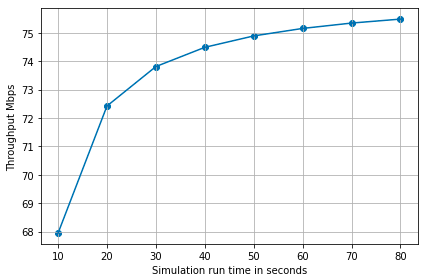
\includegraphics[width=1\linewidth]{timePlt.png}
    \caption {Throughput performance over time\vspace{-0.8em}}
    \label{fig:GeneralDiagram}
 \end{figure}

From Figure 2 below, it can be seen that all the propagation models had a throughput of 75 Mbps in about 75 meters. The throughput for FriisPropagationLossModel (FPM) remained 75 Mbps for more than 75 meters and begins to drop gradually

 \begin{figure}[h]
    \centering
    \includegraphics[width=1\linewidth]{CiDS 2021-06-10 at 20.38.43.jpeg}
    \caption {A plot showing the varying UDP throughput for five different propagation models over distance.\vspace{-0.8em}}
    \label{fig:GeneralDiagram}
 \end{figure}
 
The FixedRssLossModel Received Signal Strength (RSS) was fixed at -49 dBm and this produced a fixed throughput over 5000m and thereafter, begins to drop drastically. The lower the RSS value, the higher throughput. The throughput for ThreeLogDistancePropagationLossModel maintained 75Mbps in 75m and drop deep to about 18Mbps around 100m and thereafter, raising to 49Mbps and finally throughput started to drop gradually. TwoRayGroundPropagationLossModel (TRM) maintained similar throughput pattern as FPM to about 200m. The difference I observation between FPM model and TRM model is that FPM can cover about 30 meters more when compared with TRM.
NakagamiPropagationLossModel remained unchanged for about 2000m and thereafter begins to drop gradually.

 \begin{figure}[h]
    \centering
    \includegraphics[width=1\linewidth]{CiDS Sig 2021-06-10 at 20.41.14.jpeg}
    \caption {A plot showing the varying signal strength for five different propagation models over distance.\vspace{-0.8em}}
    \label{fig:GeneralDiagram}
 \end{figure}

As shown in Figure 3, we can see that the FRM and TRM had the same signal strength up till around 175m and thereafter, TRM had zero signal while FRM had signal up till 225m and later drop to zero. FixedRssLossModel and NakagamiPropagationLossModel had fixed signal strength for over 2000m as compared to the throughput. ThreeLogDistancePropagationLossModel had signal strength till 225m and drop to zero.

\section{Summary \vspace{-0.2em}}
FixedRssLossModel and NakagamiPropagationLossModel is observed to be good for long distance coverage while FriisPropagationLossModel, TwoRayGroundPropagationLossModel and ThreeLogDistancePropagationLossModel can be turned to be effective for short distance coverage.

\subsection*{References \vspace{-0.2em}} 
\setlength{\parindent}{0em}
[1] TechTarget, Definition of ad-hoc-network, \href{https://searchmobilecomputing.techtarget.com/definition/ad-hoc-network}{https://searchmobilecomputing.techtarget.com
/definition/ad-hoc-network}

[2] M. Stoffers and G. Riley, "Comparing the ns-3 Propagation Models,” 2012 IEEE 20th International Symposium on Modeling, Analysis and Simulation of Computer and Telecommunication Systems, Washington, DC, 2012, pp. 61-67, doi: 10.1109/MASCOTS.2012.17

[3] NS3, Flow Monitor, \href{https://www.nsnam.org/docs/models/html/flow-monitor.html}{https://www.nsnam.org/docs/models/html/flow-monitor.html}

[4] Stoffers, M., \& Riley, G. (2012, August). Comparing the ns-3 propagation models. In 2012 IEEE 20th International Symposium on Modeling, Analysis and Simulation of Computer and Telecommunication Systems (pp. 61-67). IEEE.

\end{document}
